\chapter{Introduction to the data analysis program \SASfit}

Small-angle scattering (SAS) is one of the powerful techniques to
investigate the structure of materials on a mesoscopic length scale
(10 - 10000 {\AA}). It is used to study the shapes and sizes of the
particles dispersed in a homogenous medium. The materials could be a
macromolecule (biological molecule, polymer, micelle, etc) in a
solvent, a precipitate of material A in a matrix of another material
B, a microvoid in certain metal or a magnetic inhomogeneity in a
nonmoagnetic material. This technique is also used to study the
spatial distribution of particles in a medium, thus providing the
information about the inter-particle interactions. The small angle
scattering methods includes small angle neutron, x-ray or light
scattering. The type of samples that can be studied by scattering
techniques, the sample environment that can be applied, the actual
length scale probed and the information that can be obtained, all
depend on the nature of the radiation employed. The advantage of
small-angle neutron scattering (SANS) over other SAS methods is the
deuteration method. This consists in using deuterium labeled
components in the sample in order to enhance their contrast. Whereas
SANS has disadvantaged over small-angle x-ray scattering (SAXS) by
the intrinsically low flux of neutron sources compared to the orders
of magnitude higher fluxes of x-ray sources. Neutron scattering in
general is sensitive to fluctuations in the density of nuclei in the
sample. X-ray scattering is sensitive to inhomogeneities in electron
densities whereas light scattering is sensitive to fluctuations in
polarizability (refractive index). In general, irrespective of the
type of radiation, they also share several similarities. Perhaps the
most important of these is the fact that, with minor adjustments to
account for the different types of radiation, the same basic
equations and laws can be used to analyze data from these
techniques. The small-angle scattering data can contain information
concerning both the structure and interaction within the sytem. This
information can be obtained by either performing model-independent
analysis or detailed model dependent analysis. \SASfit is such a
software package built for analysis of small-angle neutron
scattering data concerning soft matter. The main emphasis of the
software is to provide easy to use visual interface for the new as
well as for an expert user. The software package contains most of
the tools to treat large range of scientific problems and large
volume of data produced on a SAS instrument. It allows users to
derive useful information from the SAS scattering data.

\section{System Requirements And Software Installation}

{\tt SASfit} is a program for analyzing small angle scattering data.
The numerical fitting routines are written in C and the menu
interface in {\tt tcl/tk}. For the plotting of the data the {\tt
tcl} extension {\tt blt} has been used. The last version 0.85 of
{\tt SASfit} has been tested with the {\tt tcl/tk} version 8.3 and
the {\tt blt} version 2.4s. \\

\noindent
\SASfit is available for users analysing data taken at PSI. \\
\SASfit has been developed at the Paul Scherrer Institute (PSI) and remains \copyright\ of PSI. \\
\SASfit is provided to users of the PSI facilities.\\
\SASfit is provided "as is", and with no warranty. \\

\section{Installation Procedure} ~\\

\verb"SASfit" has has been compiled with tcl/tk 8.4 and Blt 2.4. To
install the \texttt{SASfit} package one has to do the following:
\begin{enumerate}
\item Download the zip-file "sasfit.zip" from the \texttt{SASfit}-home page\\
\verb"http://kur.web.psi.ch/sans1/SANSSoft/sasfit.html"
\item extract the contents of the zip file. A new subdirectory called \verb"sasfit" will be generated, which contains all required files.
\item Execute the program  \texttt{./sasfit/sasfit.exe}
\end{enumerate}

\chapter{Quick Start Tour}

\section{User Interface Window}
\begin{figure}[htb]
\centering
  \subfigure[main window]{\label{fig:QTmainA}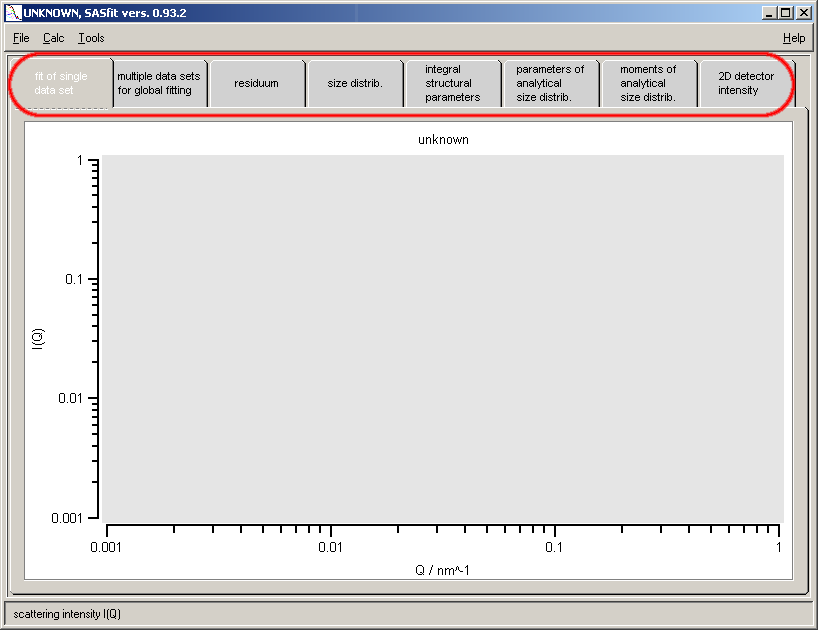
\includegraphics[width=0.48\textwidth]{QTmainA.png}}
  \subfigure[popup menu]{\label{fig:QTmainB}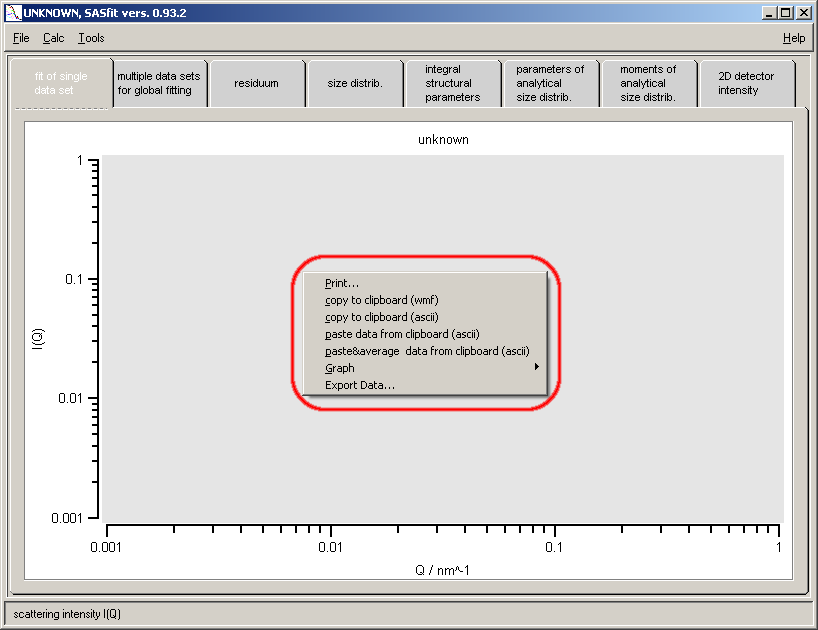
\includegraphics[width=0.48\textwidth]{QTmainB.png}}
\caption{Main \SASfit graphical user interface window}
\label{fig:QTmain}
\end{figure}
\sloppy
The core \SASfit window consists of various tabs (shown in the oval
marking in the figure \ref{fig:QTmain}(a), they are "\texttt{fit of single data set}",
"\texttt{multiple data sets for global fitting}", "\texttt{residuum}", "\texttt{size
distrib.}", "\texttt{integral structural parameters}", "\texttt{parameters of
analytical size distrib.}", "\texttt{moments of analytical size
distrib.}", and "\texttt{2D detector intensity}" as shown in the red oval
selection. The tabs for single data set and multiple data sets are used to
plot single or multiple data files and view the plotted graphs along
with the operations to perform during fitting. Residuum shows the
difference between the experimental and theoretical fits. Size
distributions give the plotted view of the number density v/s radius
of the particle. Integral structural parameters are obtained using
model independent fitting, such as Guinier approximation, Porod law
etc. Parameters of analytical size distributions provides with
details of size distributions used and the numbers obtained, whereas
moments of analytical size distribution shows the contribution of
scattering from different size distribution. The final tab 2D
detector intensity is used in case of anisotropic scattering data.
The window were the graphs are generated has options of printing the
graph plotted view, copying the data in the ASCII format or as an
image (wmf) format for further processing or presenting (figure
\ref{fig:QTmain}(b)). \SASfit accepts the isotropic data in the ASCII
format. The data can be imported as a single data set or for
multiple data sets (several scattering curves).

\section{Importing data files for a single data set}
\begin{figure}[htb]
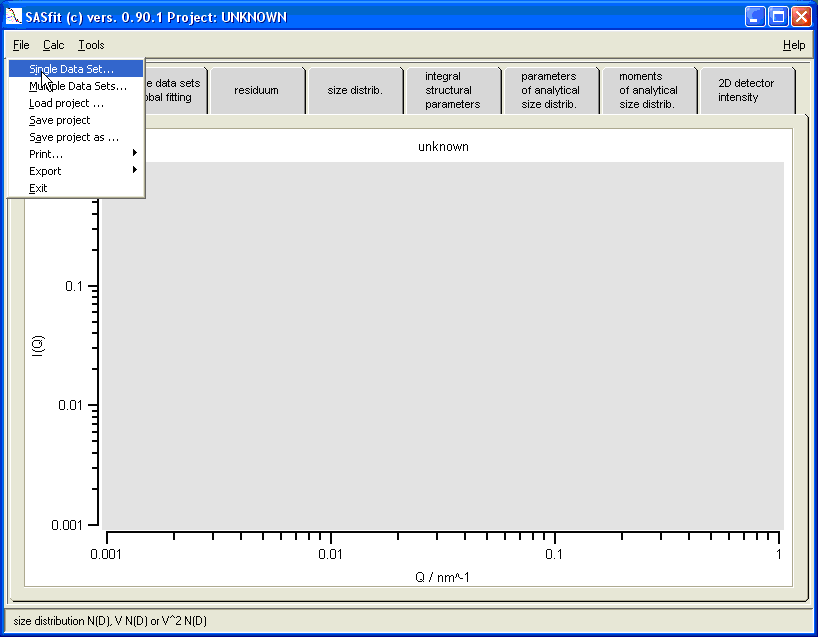
\includegraphics[width=0.48\textwidth]{QTloadingSingleDS.png}
\caption{Menu interface for input single data set}
\label{fig:QTloadingSingleDS}
\end{figure}

\begin{figure}[htb]
\centering
  \subfigure[Path and format selection for new file]{\label{fig:QTNewFile}
             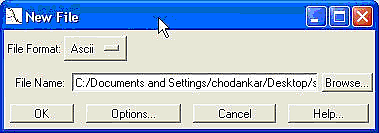
\includegraphics[width=0.44\textwidth]{QTNewFile.png}}
  \subfigure[Selecting the format columns of the file]{\label{fig:QTascii1}
             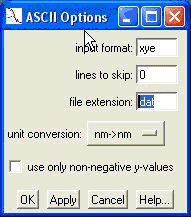
\includegraphics[width=0.22\textwidth]{QTascii1.png}
             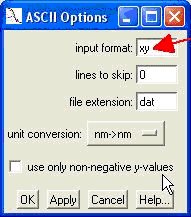
\includegraphics[width=0.22\textwidth]{QTascii2.png}}
\caption{Importing single data sets} \label{fig:QTNewFileDS}
\end{figure}

The single data set option allows the user to perform operation on a
single data file only. The file is imported via,
\verb"[File|Single Data Set...]" (Figure \ref{fig:QTloadingSingleDS}).
This will open a new file window as shown in figure
\ref{fig:QTNewFileDS}(a). The location of the file could be browsed
and respectively selected. The options buttons is supplied to select
the input format, which is performed by supplying a string such as
\texttt{xye}. Where \texttt{x}, \texttt{y} and \texttt{e} stands for
the scattering vector $Q$, scattering intensity $I(Q)$, \texttt{e}
signifies the error bar $\Delta I(Q)$ on the measured scattering intensity.
The error bars are required during the fitting operation and for files
which do not contain the error bar column it would be calculated by
default from the smoothing of the curve. There is an option to skip
lines at the beginning of the data, which is intended to be used to
skip header information in a data file , which could be misinterpreted
as data. The number $n$ specified in the menu defines the number of
lines skipped at the beginning of the data file.
Furthermore a file extension can be provided, unit conversions can be
performed as well as only non-negative $y$-values could be selected
for plotting and performing further analysis. On pressing ok the
data is loaded and the graph is plotted, with a new window labeled
merge files being opened.


\begin{figure}[htb]
\centering
  \subfigure[Merge window for merging different $Q$ scales into a single profile]{\label{fig:QTmergeSDS1}
             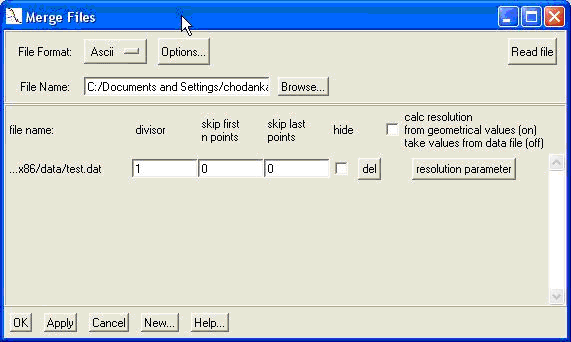
\includegraphics[width=0.5\textwidth]{QTmergeSDS1.png}}
  \subfigure[An example showing merged data files]{\label{fig:QTmergeSDS2}
             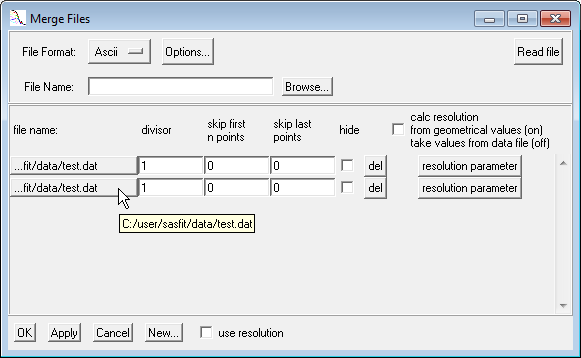
\includegraphics[width=0.5\textwidth]{QTmergeSDS2.png}}
  \subfigure[resolution parameter interface]{\label{fig:QTmergeRes}
             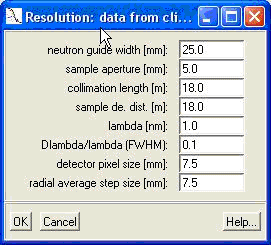
\includegraphics[width=0.3\textwidth]{QTmergeRes.png}}
\caption{Merging many data files to one data set} \label{fig:QTmergeSDScapt}
\end{figure}

In SAS, data can be collected at different collimator and sample to
detector distances to correspond for a wide $Q$ scale. Thus for a
single sample at a given condition there can be more than one data
files, to merge all of them together for completing the scattering
profile, the above shown window comes into play. As shown in the
merge files window, the new file could be browsed and selected; it
has to be read using the read file button. The newly read file
is listed below the first file, if it's a wrong selection it could
be deleted back, also one can scale the different files measured at
different $Q$ windows, using the divisor column to have a continuous
scattering profile. After scaling all the data profiles into one
single profile, the statistically bad and unwanted data points can
be removed by skipping the points at the beginning and at the end of
the data files. The resolution parameters can be provided by
pressing the resolution button and the required information such as
sample to detector distance, collimation distance, cross section of
the guide etc as shown in figure  \label{fig:QTmergeSDScapt}(c) has to be entered to use
resolution smearing during the fitting. The new button is use to
discard all the current selections and plotted data files and starts
a new session. The file could also be imported by pasting the
clipboard data on the graph view as shown in the figure below. The
conditions for columns are same as that for reading the file via
browse method.


\section{Importing data files for multiple data sets}
\begin{figure}[htb]
\centering
    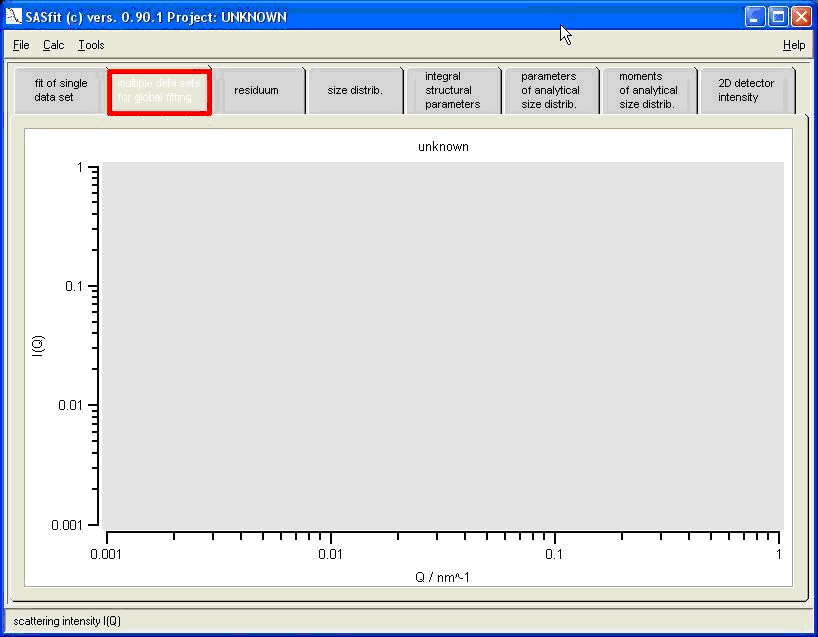
\includegraphics[width=0.49\textwidth]{QTloadingMultipleDS1.png}
    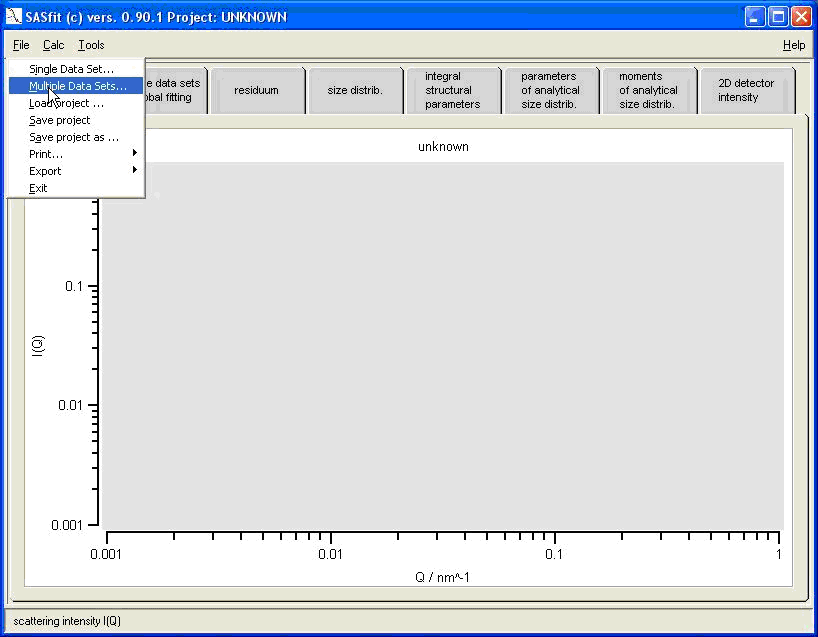
\includegraphics[width=0.49\textwidth]{QTloadingMultipleDS2.png}
\caption{Procedure for importing data files for multiple data sets}
\label{fig:QTmergeMultipleDS1}
\end{figure}
The multiple data set option allows the user to perform operation on
multiple data files by using common set of (global) parameters. This
option is especially important in contrast variation experiments or
measurements with polarized neutrons. The global fit helps to
determine the fit parameters unambiguously which by analyzing a
single curve would be otherwise strongly correlated. The file is
imported by first going to multiple data sets for global fitting
(red box in Figure \ref{fig:QTmergeMultipleDS1}) and then via,
\verb"[File|Multiple Data Set...]". This will open a new window
as was the case for importing single data set
as shown below.
\begin{figure}[htb]
\centering
  \subfigure[Path and format selection for new file ]{\label{fig:QTloadingMultipleDS3}
             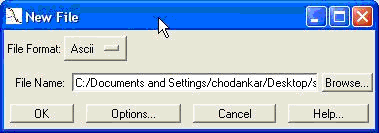
\includegraphics[width=0.6\textwidth]{QTloadingMultipleDS3.png}}
  \subfigure[Selecting the format of the file]{\label{fig:QTloadingMultipleDS4}
             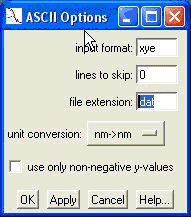
\includegraphics[width=0.3\textwidth]{QTloadingMultipleDS4.png}}
  \subfigure[Merge window for input of multiple data sets. Red box shows the buttons
             from which additional data files could be imported.
             Whereas the features of merging the data set for different $Q$ scales
             is similar to that for importing single data set]{\label{fig:QTloadingMultipleDS5}
             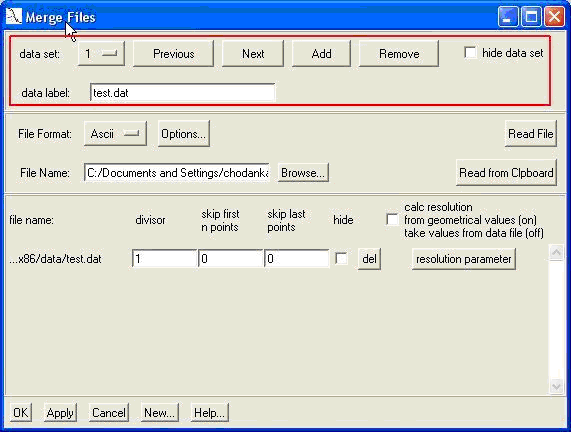
\includegraphics[width=0.7\textwidth]{QTloadingMultipleDS5.png}}
\caption{Procedure for importing data files for multiple data sets}
\label{fig:QTmergeMultipleDS2}
\end{figure}
The procedure for importing the first file is same as was the case
for single file. On reading the first file the merge file window
opens, which has additional buttons as compared to the merge file
window in single data set (shown in the red rectangular box in
figure \ref{fig:QTmergeMultipleDS2}(c)). In multiple data fitting,
almost any number of data files could be loaded. The present active
number of data is shown next to the data set in the merge file
window. One can switch over from one data file to another by
clicking previous or next. Add and remove buttons are used to add or
remove another file. The addition of curves for different $Q$ scales
is performed similar to as mentioned in the Input single data set


\section{Reducing the number of data points}

\SASfit is calculating the intensity for each data point. To make the minimization faster it can be useful to reduce the number of data points. A reduction of data points make sense if they are oversampled, i.e. within the distance of neighbouring q-values the intensity is only changing little. \SASfit supplies two algorithms for reducing the number of data points and one algorithm which is averaging data points.
After reading a data file a new entry is generated in the GUI, see e.\ g.\  \ref{fig:QTmergeMultipleDS2}(c). The filename button activates the GUI (see fig.\ \ref{fig:DataReductionOption}) for choosing an algorithm to reduce optionally the number of data points. Three procedures are supplied at the moment:
\begin{enumerate}
\item averaging neighbouring data points depending on error bar and q difference
\item skipping equally data points to reduce their numbers to a certain percentage
\item skipping nearby data points
\end{enumerate}
 By using the first option an averaging of data points $I_k(q_k) \ldots I_l(q_l)$ is done as long as they fulfill the conditions that
\begin{align}
\forall n \in (k,l] : \abs{I_k-I_n} < D_\mathrm{min} (\Delta I_k + \Delta I_n)
\quad \bigwedge \quad \abs{q_k-q_n}/\overline{q} <  \Delta q_{max}
\end{align}
where $D_\mathrm{min} $ and $\Delta q_{max}$ are user supplied values. 
The averaging of data points therefore depends on a user-defined maximum allowed $q$-smearing $\Delta q_{max}$ and  a user-defined maximum distance in intensity in units of the error bar ($D_\mathrm{min} $), so that an averaging is only performed, if the intensities look similar with $D_\mathrm{min}$-times the intensity error bars and are not to far away from each other on the q-axes.
The second option simply skips data points equally to reduce the amount data. The parameter "percentage/100 to load" defines the amount of data to be kept. A value of 1 means all data are kept and a value of 0.5 means every second data point will be kept. In the third option one can define a distance in the $q:I(q)$-plot or $\log q: \log I(q)$ plot. The next data point, which will be plotted must have either in the linear or logarithmic plot a distance exceeding a user defined value.
 
\begin{figure}[htb]
\centering
  \subfigure[Averaging data points depending on the error bar and resulting resolution.]{\label{fig:DataReductionOptionAVG1}
             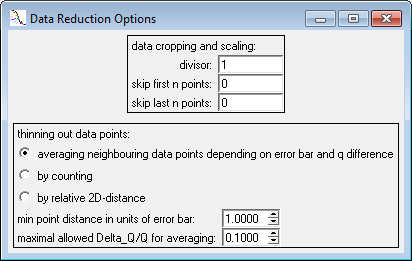
\includegraphics[width=0.3\textwidth]{../images/GUI/DataReductionOptionAVG1.png}}
  \subfigure[skipping data points to reduce the number of points to a certain amount.]{\label{fig:DataReductionOptionSKIP1}
             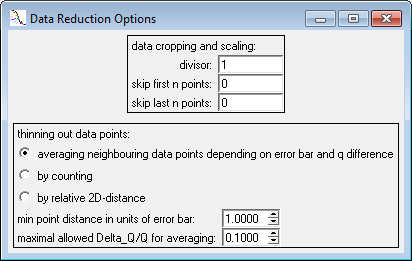
\includegraphics[width=0.3\textwidth]{../images/GUI/DataReductionOptionAVG1.png}}
  \subfigure[reducing the number of data points by defining a minimum distance between them to be plotted.]{\label{fig:DataReductionOptionSKIP2}
             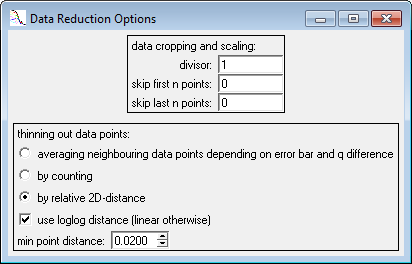
\includegraphics[width=0.3\textwidth]{../images/GUI/DataReductionOptionSKIP2.png}}
\caption{GUI for input values of the two algorithms for reducing the number of data points and for one algorithm which is averaging data points.}
\label{fig:DataReductionOption}
\end{figure}

\section{Simulating scattering curves}

In addition to reading and loading data set, one can also have a
realistic view of the experimental scattering data for a known
structure by simulating the scattering profile beforehand to get a
feel of the actual experiment scattering profile. The simulation can
be performed either for a single data set or for multiple data sets
using global parameters. To generate theoretical scattering profile,
follow \verb"[Calc|Single Data Set...|simulate]" or
\verb"[Calc|Multiple Data Sets...|simulate]", either of them to generate
a single data set or multiple data sets varied by changing the global parameter. The
data can be generated for vast number of form factors and structure
factor included in the software. The simulation is calculated using
physically relevant parameters, this is useful to plan the
experiment and to know whether a given concentration and contrast
would produce a measurable signal.

\begin{figure}[htb]
\centering
  \subfigure[simulation of a single curve]{\label{fig:QTsimulateSDS}
             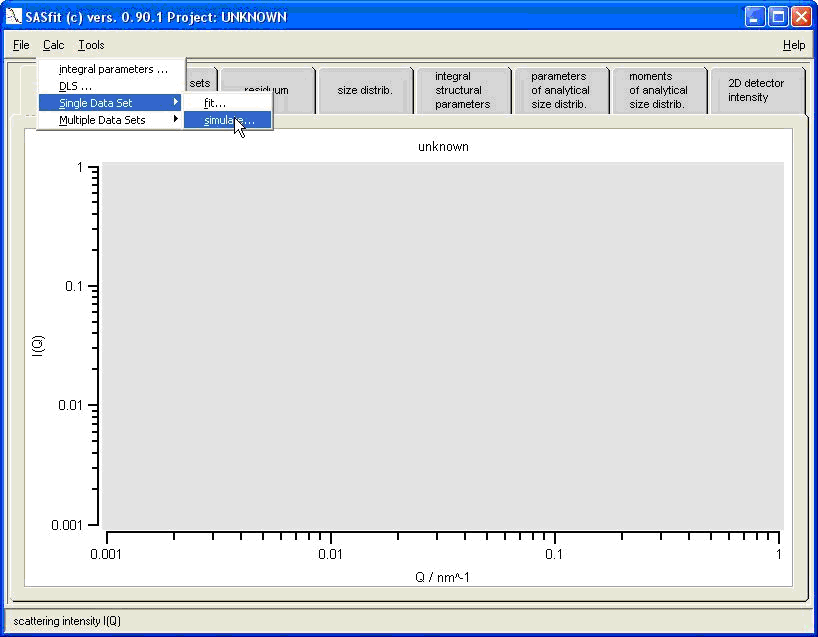
\includegraphics[width=0.48\textwidth]{QTsimulateSDS.png}}
  \subfigure[simulation of multiple curves]{\label{fig:QTsimulateMDS}
             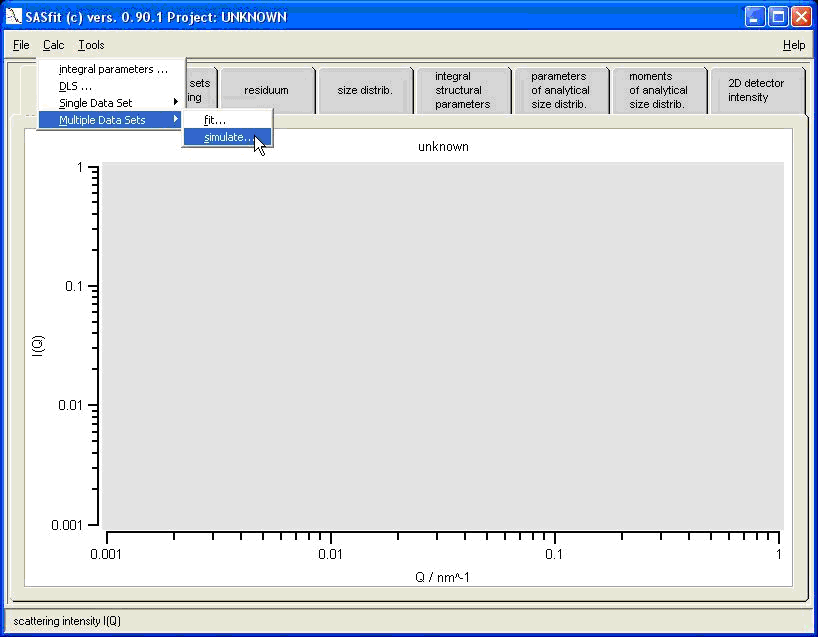
\includegraphics[width=0.48\textwidth]{QTsimulateMDS.png}}
\caption{Procedure for simulating data profiles for single as well as multiple data files}
\label{fig:QTsimulateDS}
\end{figure}

\section{Fitting}
\SASfit can analyse the data using both model-independent analysis
and using a non-linear least square method to fit models. The
model-independent analysis is a preliminary process of analyzing SAS
data and does not require any advanced knowledge of the system to
extract structural information this includes fittings (Guinier,
Kratky, Porod, power-laws, etc.). On the other hand in case of
non-linear least square methods a detailed fitting to the
experimental data is performed using a wide variety of form factors
and structure factors. The \SASfit model library consists of large
number of such functions, which can be readily used for the
analysis. Moreover it can also fit different size distributions.

\subsection{Model Independent Fitting (Integral parameters)} ~\\
Model independent analysis requires no advanced knowledge about the
sample and most importantly no experimental bias of assumed
structure. It includes linearized fitting (Guinier, Porod and Zimm
plot) to extract structural information. Model independent analysis
are performed via \verb"[Cals|integral parameters]". In \SASfit
there are basically three functions available to do the analysis;
they are Guinier, Zimm and Porod approximations (shown in the blue
box in Figure \ref{fig:QTintegralparameter}(b). The number of data points to be included in the
analysis can be accordingly varied and the resulting fit and the
available parameters can be viewed instantaneously. For a large
number of data a small script can be return to automate the process.
This is performed by using the lower section of the integral
structural parameters window (shown in red box). Prename indicates a
character or string of characters with which all the data file names
to be analysed starts with followed by certain numbers. The number
of digits/characters in the filename could be given in the digits
submission box, whereas the start number and the last file number
are provided in their respective submission boxes. The step box
indicates the incremental step of the file names which has to be
analysed. The fitted parameters can be saved in the custom file to
be viewed later. Load next file does step by step analysis of
different files, whereas Do all would perform calculations on the
entire file list, to be saved in the custom file for later viewing.

\begin{figure}[htb]
\centering
  \subfigure[data with fit results]{\label{fig:QTintegralparameterTab}
             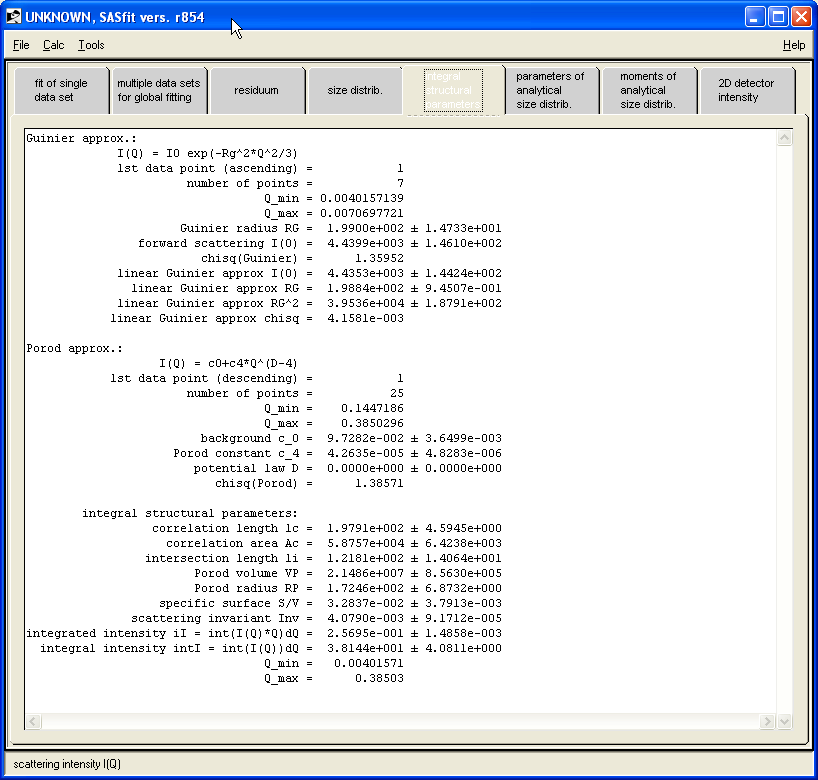
\includegraphics[width=0.48\textwidth]{QTintegralparameterTab.png}}
  \subfigure[entry menu with fitted parameters]{\label{fig:QTintegralparameterMenu}
             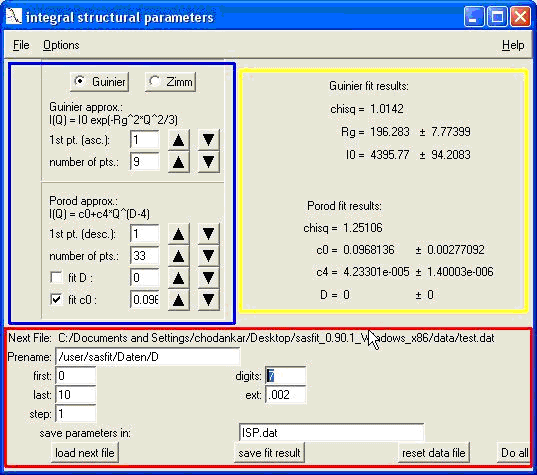
\includegraphics[width=0.48\textwidth]{QTintegralparameterMenu.png}}
\caption{Integral fit parameters}
\label{fig:QTintegralparameter}
\end{figure}

A set of valuable size and integrated parameters that can be
calculated directly from the scattering curves $I(Q)$
\cite{Damaschun1969,Sjoberg1974,Damaschun1971,Walter1985,Moller1995,book:Guinier:Fournet}
consists of
\begin{subequations}
\begin{align}
\tilde{Q}_\text{inv} &= \int_0^\infty Q^2I(Q) \mathrm{d}Q \mbox{ (scattering invariant)} \\
\frac{S}{V} &= \frac{\pi}{\tilde{Q}_\text{inv}} \;\; {\DS\lim_{Q \to \infty}\left\{Q^4I(Q)\right\}} \mbox{ (specific surface)} \\
\langle R_G \rangle^2 &= 3\left(-\DS\lim_{Q \to 0}\left\{\frac{\mathrm{d}[\ln I(Q)]}{\mathrm{d}(Q^2)}\right\}\right) \mbox{ (squared Guinier radius)} \\
\langle d \rangle &= \frac{4}{\pi}\frac{\int_0^\infty Q^2I(Q) \mathrm{d}Q}{\DS\lim_{Q \to \infty}\left\{Q^4I(Q)\right\}} \mbox{ (average intersection length)} \\
\langle l \rangle &= \frac{\pi}{\tilde{Q}_\text{inv}} \int_0^\infty QI(Q) \mathrm{d}Q \mbox{ (correlation length)} \\
\langle A \rangle &= \frac{2\pi}{\tilde{Q}_\text{inv}}\int_0^\infty I(Q) \mathrm{d}Q \mbox{ (correlation surface)} \\
\langle V \rangle &= \frac{2\pi^2}{\tilde{Q}_\text{inv}} I(0) \mbox{ (correlation volume, Porod volume)}
\end{align}
\end{subequations}

\subsection{Model dependent analysis}
\subsubsection{Modeling a single data set}~\\
\begin{figure}[htb]
\centering
  \subfigure[Menu through which fitting procedure is initiated]{\label{fig:QTsinglefitTab}
             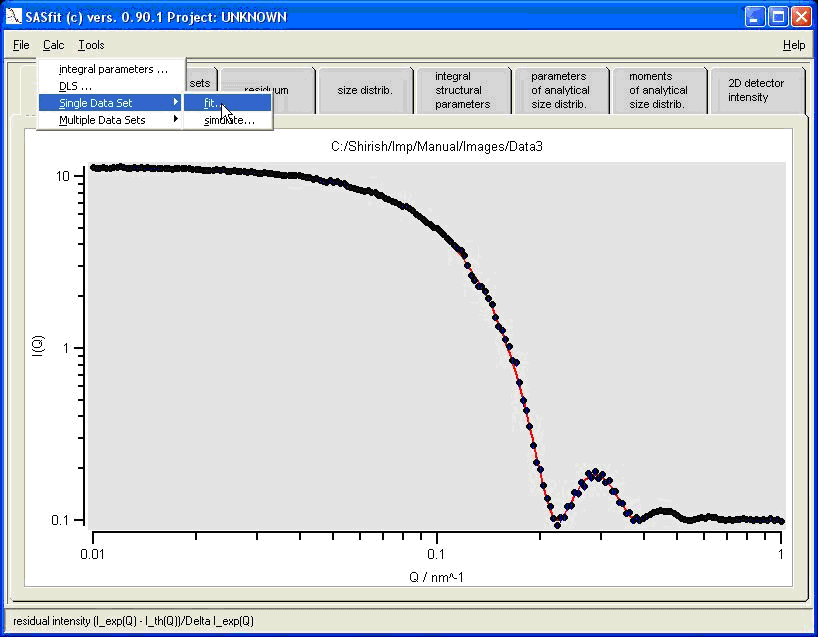
\includegraphics[width=0.5\textwidth]{QTsinglefit1.png}}
  \subfigure[User interface for fitting, containing different form factors and structure factor]{\label{fig:QTsinglefitEntryMenu}
             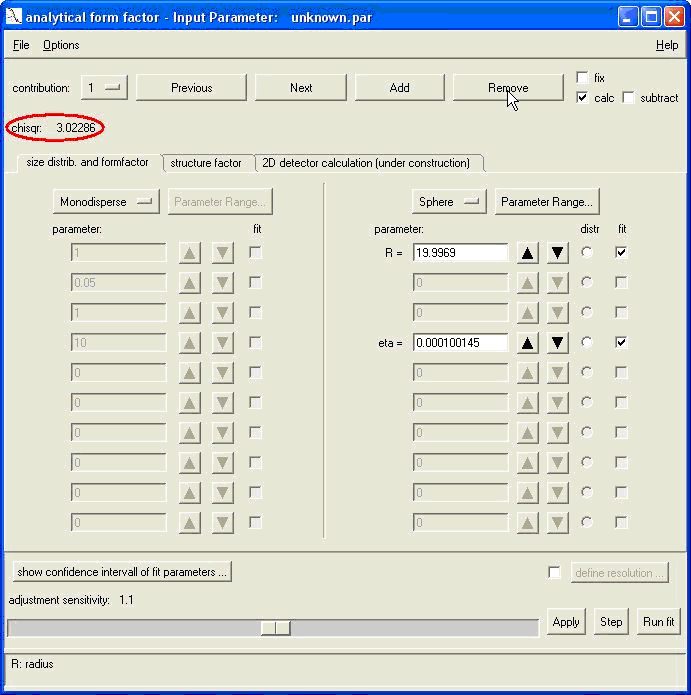
\includegraphics[width=0.48\textwidth]{QTsinglefit2.png}}
  \subfigure[Tab summarizing the analyzed parameters]{\label{fig:QTsinglefitParOverview}
             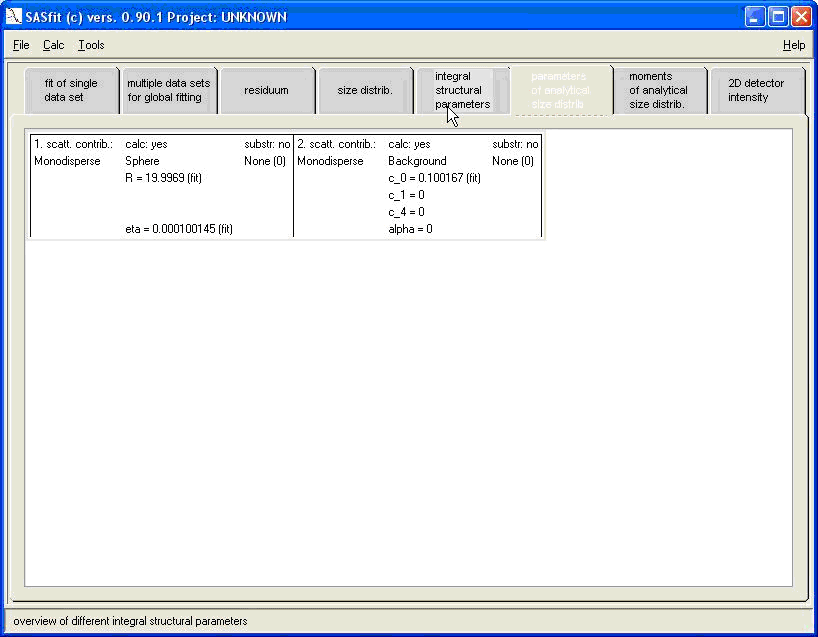
\includegraphics[width=0.48\textwidth]{QTsinglefit3.png}}
\caption{Menus for fitting a single data set}
\label{fig:QTsinglefit}
\end{figure}
For Modeling a SANS data set the \SASfit-programm allows to
describe experimental data with an arbitrary number of scattering
objects types. Each of them can have a size distribution, whereby
the user can choose over which parameter $a_i$ of the form factor
the integration will be performed. For example in case of a
spherical shell with a core radius of $R$ and a shell thickness of
$\Delta R$ \SASfit allows to integrate either over the core
radius $x=R$ or the shell thickness $x=\Delta R$ by marking the
corresponding parameter (see option {\tt distr} in Fig .
\ref{fig:QTsinglefit}(b)). Furthermore an additional structure factor
can be included for each scattering object. Several ways to account
for the structure factor have been implemented like the monodisperse
approximation (\ref{sec:SQmonodisperse}), decoupling approach
(\ref{sec:SQdecoupling}), local monodisperse approximation
(\ref{sec:SQlocalmonodisperse}), partial structure factor
(\ref{sec:SQpartial}) and scaling approximation of partial structure
factors (\ref{sec:SQscaling}). The details are described in chapter
\ref{sec:structurefactor}.

Implemented size distributions, form factors and structure factors
are described in chapters \ref{formfactor},
\ref{sec:structurefactor} and \ref{sizedistribution}. Optional an
additional smearing of this function with the instrument resolution
function $R_{av}\left(Q,\langle Q\rangle\right)$ can be activated so
that
\begin{equation}
I(\langle Q\rangle) = \int_0^\infty R_{av}\left(Q,\langle
Q\rangle\right) \frac{d\sigma}{d\Omega}(Q) \, dQ
\end{equation}

A user interface shown in Fig. \ref{fig:QTsinglefit} is supplied to
choose between the number of scattering objects and to define
parameter for each of them. Next to varying the different parameters
one can mark those, which one would like to fix or to vary in a
fitting procedure (see option {\tt fit} in Fig.
\ref{analyticalMenu}(b)) Model dependent analysis for single files
are performed via \verb"[Calc|Single Data Set|Fit...]".

\subsubsection{Modeling multiple data sets}~\\
\begin{figure}[htb]
\centering
  \subfigure[Imported multiple data sets]{\label{fig:QTmultiplefit1}
             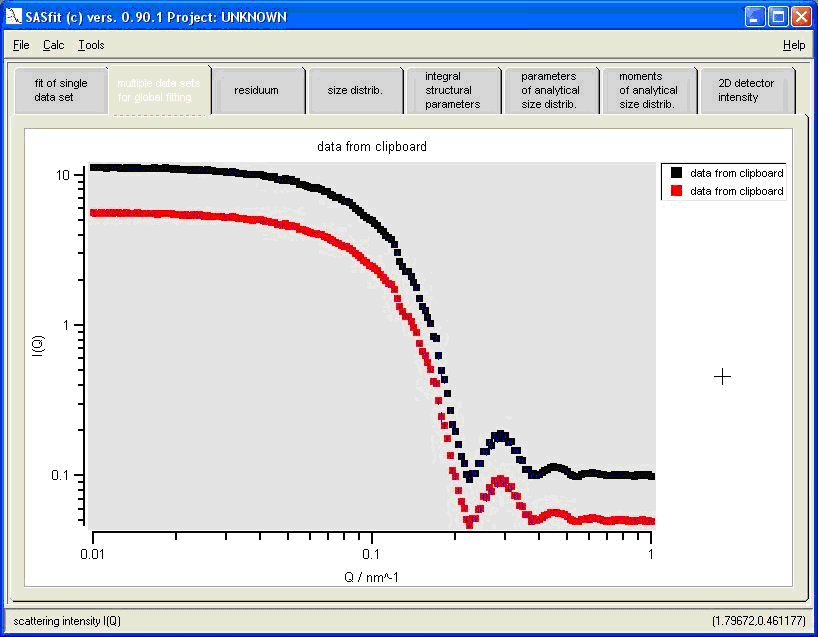
\includegraphics[width=0.48\textwidth]{QTmultiplefit1.png}}
  \subfigure[Uuser interface for fitting multiple data files]{\label{fig:QTmultiplefit2}
             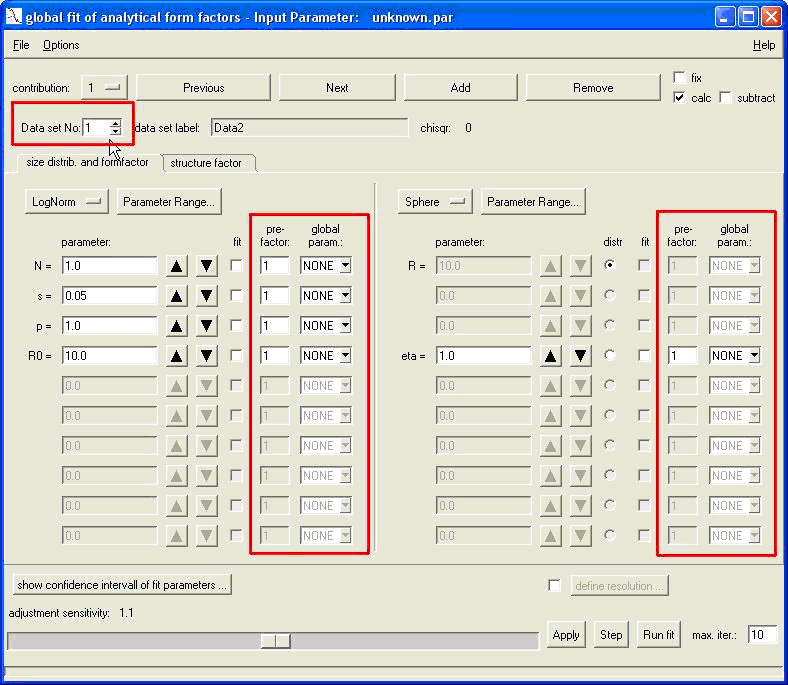
\includegraphics[width=0.48\textwidth]{QTmultiplefit2.png}}
\caption{Menus for fitting a simultaneously multiple data sets}
\label{fig:QTmultiplefit}
\end{figure}
The multiple data set option allows the user to perform operation on
multiple data file by using common set (global) parameters. This
option is especially important in contrast variation experiments or
measurements with polarized neutrons. The global fitting helps the
user to analyse large number of data which has a similar form or
structure factor however different scaling constant. The data shown
in the figure below is for a spherical monodispersed system both the
data profile has identical features, except that the scaling factor
between the two is of a factor of two. The data are called by the
procedure explained in the input multiple data file section. The
fitting of the data is performed by calling the fitting function via
\verb"[Calc|Multiple Data Sets|Fit...]". The user interface for multiple
data fitting has additional feature than to that for single data
fitting, they are pre-factor and global parameters as shown in
figure \ref{fig:QTmultiplefit}(b) red markings.


\begin{figure}[htb]
\centering
  \subfigure[]{\label{fig:QTmultiplefitUI1}
             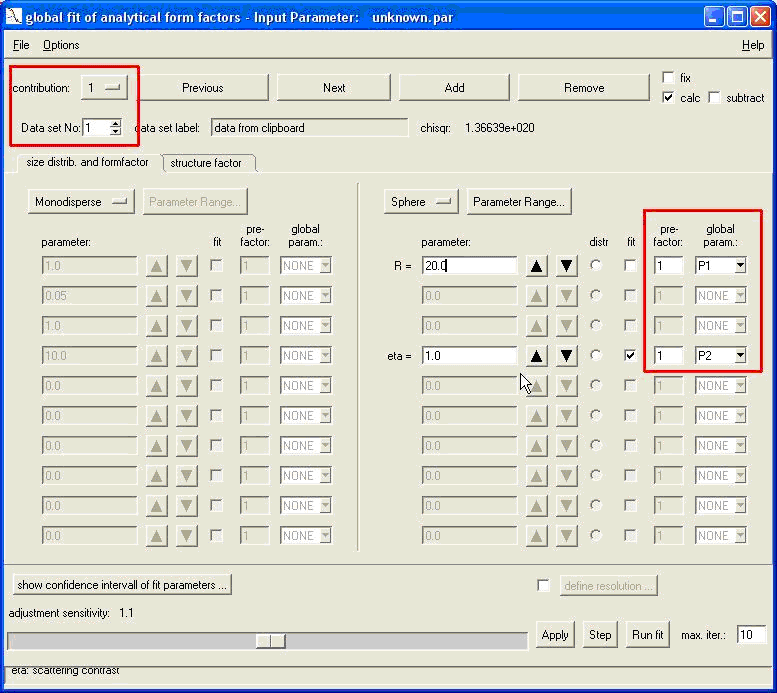
\includegraphics[width=0.48\textwidth]{QTmultiplefitUI1.png}}
  \subfigure[]{\label{fig:QTmultiplefitUI2}
             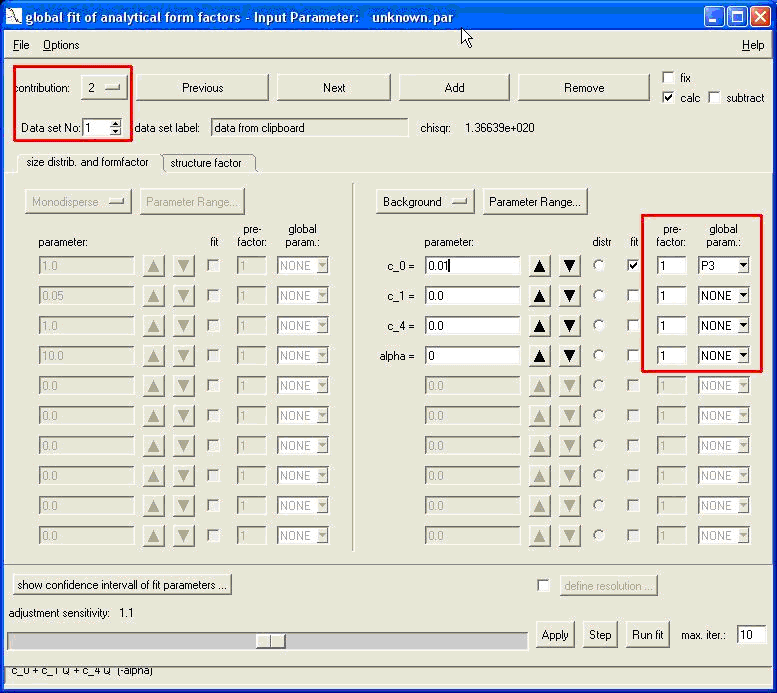
\includegraphics[width=0.48\textwidth]{QTmultiplefitUI2.png}}
  \subfigure[]{\label{fig:QTmultiplefitUI3}
             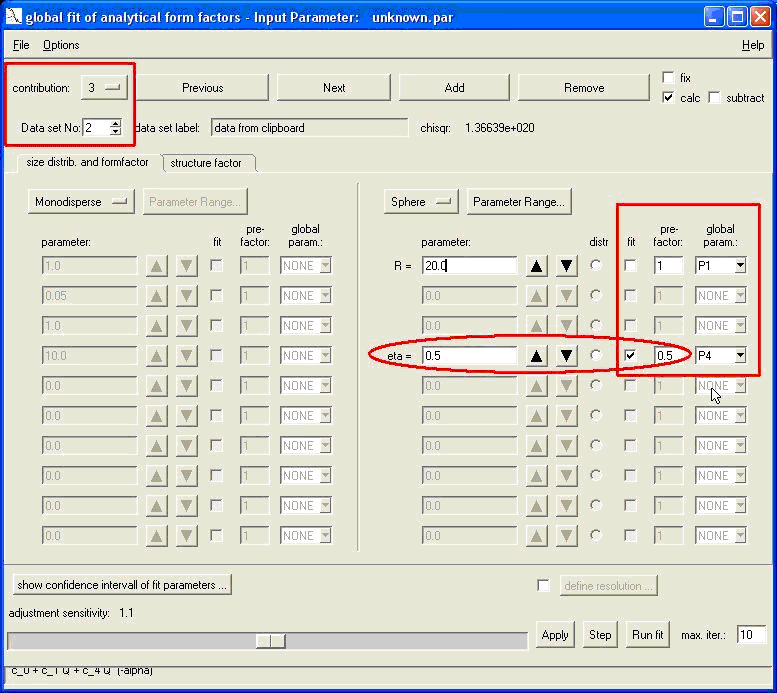
\includegraphics[width=0.48\textwidth]{QTmultiplefitUI3.png}}
  \subfigure[]{\label{fig:QTmultiplefitUI4}
             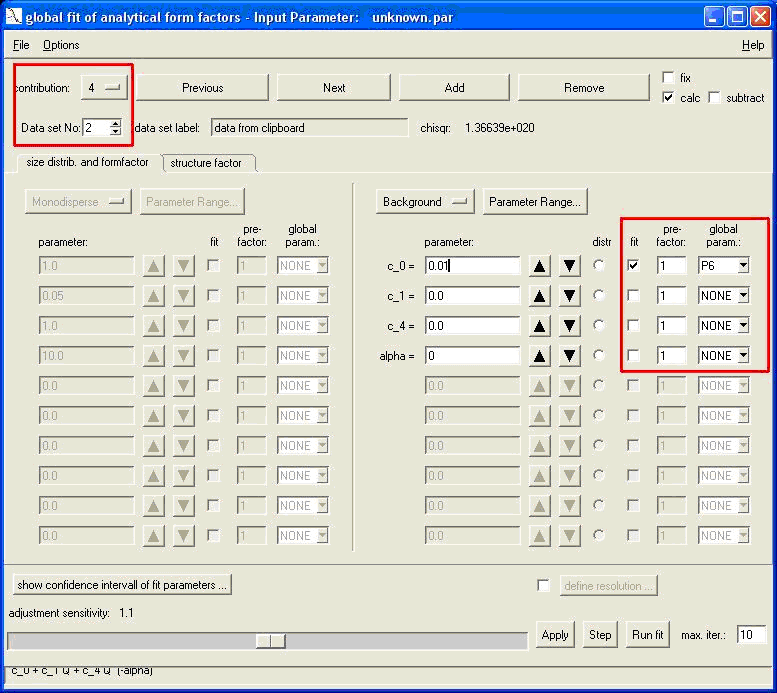
\includegraphics[width=0.48\textwidth]{QTmultiplefitUI4.png}}
\caption{Different windows showing different controlling parameters during multiple data fitting.}
\label{fig:QTmultiplefitUI}
\end{figure}

The procedure for fitting the data set is similar to that mentioned
in the earlier section. The only difference is to include the global
parameters for each function included. The scattering profile shown
in the figure \ref{fig:QTmultiplefit}(a) is for a spherical
monodispersed particle, both
the profiles have identical features with a scaling factor of two.
The user interface for fitting shows the following window in figures
\ref{fig:QTmultiplefitUI}. The data set number shows the active data file, whereas
contribution indicates the number of scattering objects. We have
selected the form factor for a spherical particle. In the global
parameter a new variable is produced for both radius and \texttt{eta}
(scattering contrast). The pre-factor is kept constant at 1. A
second contribution is added to the data set one by pressing add. In
this case it is a background contribution, a new global parameter is
introduced for it (\texttt{P3}). A similar procedure is done for second data
set where the global parameter for the radius is kept same to that
for data set one, whereas new global parameters are defined for
scattering contrast and background. The fitting procedure can then
be started by pressing Run fit. The figures \ref{fig:QTmultiplefitUIeg}
show the graphs during the fitting process. The parameters of fitting for all the
contribution can be viewed by pressing parameters of analytical size
distributions (figure \ref{fig:QTmultiplefitUIeg}(d)).

\begin{figure}[htb]
\centering
  \subfigure[]{\label{fig:QTmultiplefitUI5}
             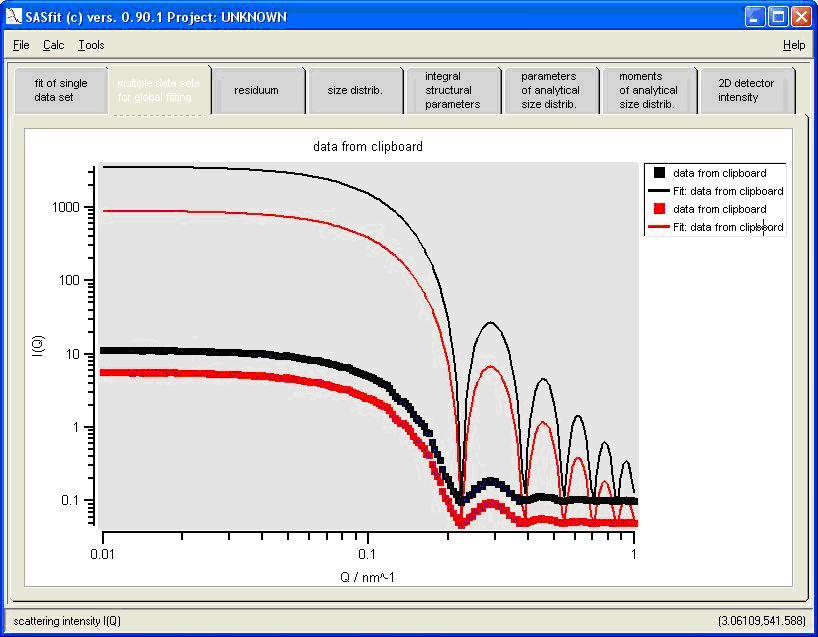
\includegraphics[width=0.48\textwidth]{QTmultiplefitUI5.png}}
  \subfigure[]{\label{fig:QTmultiplefitUI6}
             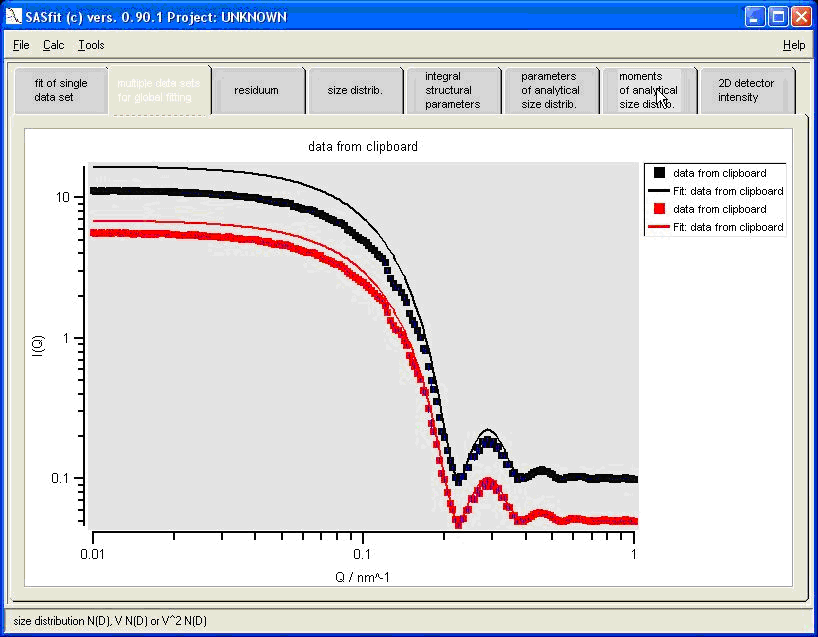
\includegraphics[width=0.48\textwidth]{QTmultiplefitUI6.png}}
  \subfigure[]{\label{fig:QTmultiplefitUI7}
             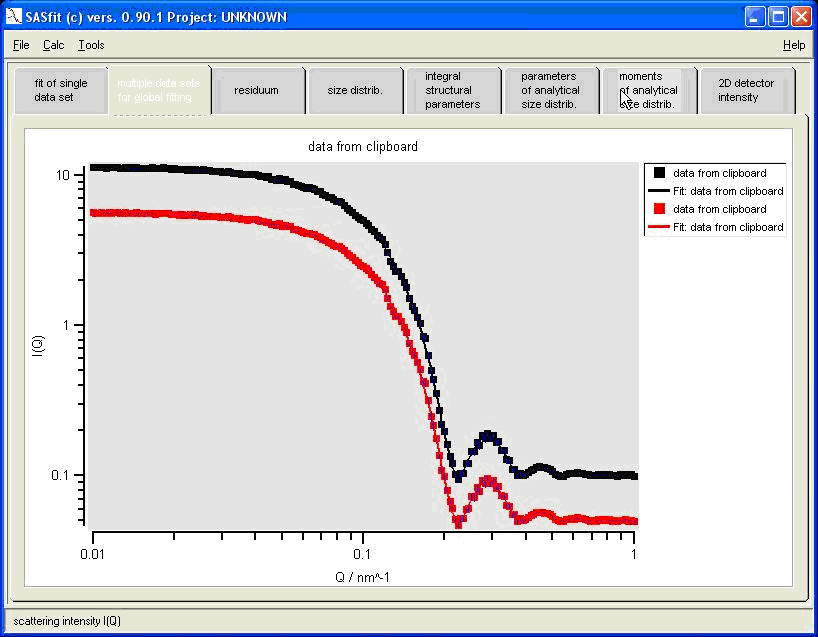
\includegraphics[width=0.48\textwidth]{QTmultiplefitUI7.png}}
  \subfigure[]{\label{fig:QTmultiplefitUI8}
             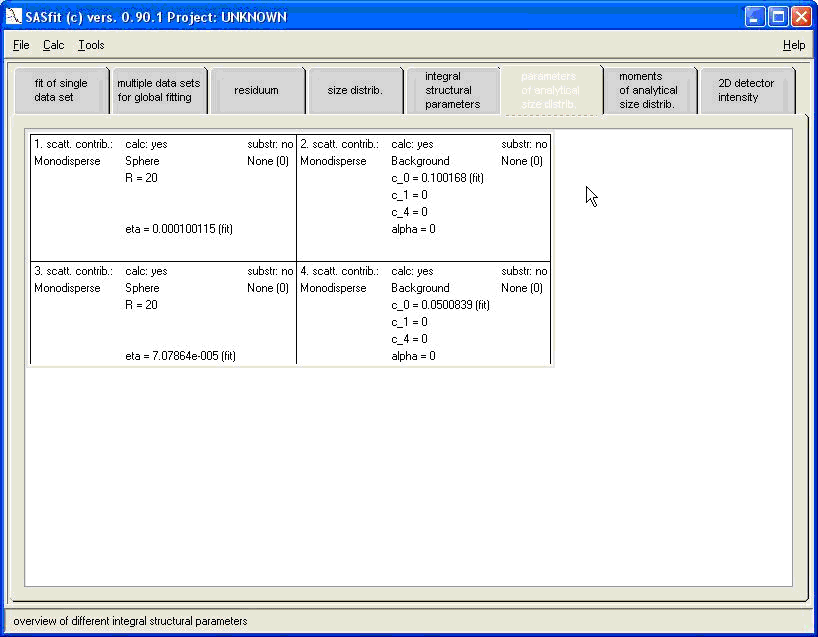
\includegraphics[width=0.48\textwidth]{QTmultiplefitUI8.png}}
\caption{The scattering data profile and the analytical parameters obtained during the fitting process.}
\label{fig:QTmultiplefitUIeg}
\end{figure}
